\documentclass[aspectratio=169,10pt,t]{beamer}
\usepackage{issa}  % place issa.sty in the same folder
\definecolor{AccentCol}{HTML}{1E7A45}
\renewcommand{\lecnum}{2}
\newcommand{\bdpts}{\foreach \x/\y in {0.4/2.4,0.9/2.0,0.6/1.5,1.2/2.6,1.5/1.8,1.0/1.0}{\node[pt1]at(\x,\y){};}\foreach \x/\y in {2.6/0.5,3.1/1.1,2.4/1.3,3.4/0.6,2.8/1.7,3.3/2.0}{\node[pt2]at(\x,\y){};}}
\begin{document}
\titleslide{2}{Supervised Learning Part 1:\\Classification Algorithms for Defence}{Logistic Regression \textbullet\ kNN \textbullet\ Decision Trees \textbullet\ Random Forest \textbullet\ SVM \textbullet\ Naive Bayes\\Case study: 5-class IADS threat classification, N = 8,500 samples, 11 radar + EW features}

\sect{1. Objectives \& Data}
\begin{frame}{Lecture 2 --- Objectives \& Dataset Overview}
\subhead{What we cover today: 6 classifiers, 1 unified dataset}
\begin{columns}[T]
\column{0.50\textwidth}
\begin{cbox}{Learning objectives}\scriptsize
\begin{te}\item Derive decision boundaries for key classifiers\item Implement logistic regression mathematically\item Understand bias--variance for kNN ($k$ effects)\item Build \& prune a decision tree from first principles\item Explain random-forest bagging \& feature importance\item Derive SVM hard \& soft margins; the kernel trick\item Apply Naive Bayes to a classification problem\item Select the right classifier for a defence scenario\item Compute precision, recall, F1, ROC-AUC from scratch\item Identify class imbalance \& apply fixes\end{te}\end{cbox}
\begin{cbox}[ISSAnavy]{Unified case study protocol}\scriptsize Each algorithm is trained on the SAME data and compared on accuracy, F1-macro, per-class precision/recall, training time \& inference latency, and decision-boundary geometry.\end{cbox}
\column{0.48\textwidth}
\subhead{5-class IADS threat dataset: $N=8{,}500$, 11 features, split 68/17/15}
\figc{1.9cm}{\bars{2000}{1.3}{1.7}{FF Friendly Fighter/1700/ISSAgrn,AB Adversary Bomber/1700/ISSAred,CM Cruise Missile/1700/ISSAblue,UV UAV-Drone/1700/violet,CI Civilian Aircraft/1700/ISSAamb}}
\figc{3.2cm}{\scriptsize\renewcommand{\arraystretch}{1.15}\begin{tabular}{lll}\toprule\textbf{Feature}&\textbf{Feature}&\textbf{Feature}\\\midrule $x_1$ Peak frequency (GHz)&$x_5$ Scan rate (deg/s)&$x_9$ EW jamming (boolean)\\$x_2$ Pulse width ($\mu$s)&$x_6$ Polarisation (categ.)&$x_{10}$ Course (deg)\\$x_3$ PRF (Hz)&$x_7$ Doppler shift (MHz)&$x_{11}$ Speed (km/h)\\$x_4$ Amplitude (dBm)&$x_8$ Sidelobe level (dBc)&\\\bottomrule\end{tabular}}
\end{columns}
\end{frame}

\sect{2. Framework}
\begin{frame}{Quick Recap --- Supervised Learning \& the Classification Framework}
\subhead{Supervised classification: the general pipeline}
\figc{1.7cm}{\begin{tikzpicture}\tikzset{S/.style={ndA,text width=2.2cm,minimum height=1.1cm}}
\node[S](a)at(0,0){\textbf{1 Feature engineering}\\z-score $\tilde x=(x-\mu)/\sigma$};\node[S](b)at(2.8,0){\textbf{2 Model training}\\$\min\sum\ell(f(x_i;\theta),y_i)+\lambda R(\theta)$};\node[S](c)at(5.6,0){\textbf{3 Hyper-parameter tuning}\\$k$-fold CV ($k=5$ or 10)};\node[S](d)at(8.4,0){\textbf{4 Test evaluation}\\held-out test set only};\node[S](e)at(11.2,0){\textbf{5 Deploy + monitor}\\watch for distribution shift};
\foreach \u/\v in {a/b,b/c,c/d,d/e}{\draw[bigarr](\u)--(\v);}\end{tikzpicture}}
\begin{columns}[T]
\column{0.50\textwidth}
\begin{cbox}[ISSAnavy]{Setup}\scriptsize Training set $D=\{(x_i,y_i)\}_{i=1}^{N}$, $x_i\in\mathbb{R}^{d}$ with $d=11$, $y_i\in\{$FF, AB, CM, UV, CI$\}$. \textbf{Never} peek at the test set during training.\end{cbox}
\begin{wbox}\scriptsize\textbf{DATA-PITFALL CHECK before training:} \textcircled{\tiny1} class balance \textcircled{\tiny2} feature scaling applied \textcircled{\tiny3} no data leakage (future information in training) \textcircled{\tiny4} categorical features encoded \textcircled{\tiny5} missing values handled.\end{wbox}
\column{0.48\textwidth}
\figc{3.3cm}{\scriptsize\renewcommand{\arraystretch}{1.2}\begin{tabular}{llcc}\toprule\textbf{Classifier}&\textbf{Type}&\textbf{Parametric}&\textbf{Needs scaling}\\\midrule Logistic reg.&Linear&Yes&\cellcolor{ISSAgrn!25}No\\kNN&Instance&No&\cellcolor{ISSAred!30}\textbf{YES}\\Decision tree&Non-linear&No&\cellcolor{ISSAgrn!25}No\\Random forest&Ensemble&No&\cellcolor{ISSAgrn!25}No\\SVM&Margin&Yes&\cellcolor{ISSAred!30}\textbf{YES}\\Naive Bayes&Probabilistic&Yes&\cellcolor{ISSAgrn!25}No\\\bottomrule\end{tabular}}
\sm{Red = mandatory feature scaling; green = scaling not required.}
\end{columns}
\end{frame}

\sect{3. Decision Boundaries}
\begin{frame}{Decision Boundaries --- Each Classifier Carves Space Differently}
\figc{2.9cm}{\begin{tikzpicture}[x=0.85cm,y=0.85cm]
\begin{scope}\draw[ISSAgrey](0,0)rectangle(4,3);\bdpts\draw[AccentCol,line width=1.2pt](1.4,0)--(2.2,3);\node[lab]at(2,-0.35){\textbf{Logistic regression}: hyperplane $w\!\cdot\!x+b=0$};\end{scope}
\begin{scope}[xshift=4.6cm]\draw[ISSAgrey](0,0)rectangle(4,3);\bdpts\draw[AccentCol,line width=1.2pt](1.9,0)--(1.7,1.0)--(2.3,1.5)--(1.9,2.3)--(2.1,3);\node[lab]at(2,-0.35){\textbf{kNN}: Voronoi, local};\end{scope}
\begin{scope}[xshift=9.2cm]\draw[ISSAgrey](0,0)rectangle(4,3);\bdpts\draw[AccentCol,line width=1.2pt](2.0,0)--(2.0,1.2)--(1.7,1.2)--(1.7,2.2)--(2.3,2.2)--(2.3,3);\node[lab]at(2,-0.35){\textbf{Decision tree}: axis-aligned staircase};\end{scope}
\begin{scope}[xshift=13.8cm]\draw[ISSAgrey](0,0)rectangle(4,3);\bdpts\draw[AccentCol,line width=1.2pt,smooth](1.6,0)..controls(2.4,1.0)and(1.5,1.9)..(2.0,3);\fill[AccentCol!15,opacity=0.5](1.6,0)..controls(2.4,1.0)and(1.5,1.9)..(2.0,3)--(4,3)--(4,0)--cycle;\node[lab]at(2,-0.35){\textbf{SVM / RBF}: smooth max-margin};\end{scope}
\end{tikzpicture}}
\begin{columns}[T]
\column{0.50\textwidth}
\begin{tl}\item \textbf{Logistic:} works when classes are linearly separable\item \textbf{kNN:} any shape; noisy near boundaries\item \textbf{Tree:} interpretable but straight-edged only\item \textbf{SVM/RBF:} optimal generalisation via kernels\end{tl}
\column{0.48\textwidth}
\begin{rbox}\scriptsize\textbf{IADS context:} in our 11-D feature space a ``decision boundary'' is a hyperplane or hypersurface separating 5 class regions. Linear = 5 hyperplanes (one-vs-rest); RBF-SVM finds a curved separating surface.\end{rbox}
\end{columns}
\end{frame}

\begin{frame}{Bias--Variance Trade-off and the Evaluation Protocol}
\begin{columns}[T]
\column{0.50\textwidth}
\subhead{Bias--variance trade-off}
\figc{2.9cm}{\begin{tikzpicture}[x=0.65cm,y=0.65cm]
\foreach \xo/\ttl/\cl in {0/HIGH BIAS (underfit)/ISSAred,4.4/GOLDILOCKS ZONE/ISSAgrn,8.8/HIGH VARIANCE (overfit)/ISSAamb}{\begin{scope}[xshift=\xo cm]\draw[ISSAgrey](0,0)rectangle(4,3);\bdpts\node[font=\fontsize{5.5}{6}\selectfont\bfseries,\cl]at(2,3.3){\ttl};\end{scope}}
\draw[AccentCol,thick](0.3,2.8)--(3.7,0.2);
\draw[AccentCol,thick,smooth](4.7,2.9)..controls(6.0,1.7)and(6.6,1.8)..(8.2,0.1);
\draw[AccentCol,thick](8.8,2.9)--(9.4,2.0)--(9.8,2.6)--(10.4,1.3)--(10.8,1.9)--(11.2,0.7)--(11.9,1.4)--(12.5,0.2);
\end{tikzpicture}}
\begin{tl}\item \textbf{High bias:} too simple, wrong even on training data (straight line for a curved boundary; LR on non-linear data)\item \textbf{High variance:} perfect on train, fails on test (deep tree, 1-NN)\item \textbf{Goldilocks:} low bias + low variance --- found by cross-validation\end{tl}
\column{0.48\textwidth}
\subhead{Evaluation protocol: train $\to$ tune $\to$ test}
\figc{2.0cm}{\begin{tikzpicture}[x=0.9cm]
\foreach \fk in {1,...,5}{\node[font=\fontsize{5.5}{6}\selectfont,anchor=east]at(-0.1,-\fk*0.33){Fold \fk};\foreach \fj in {1,...,5}{\fill[ISSAblue!50](\fj-0.5,-\fk*0.33-0.12)rectangle(\fj+0.45,-\fk*0.33+0.12);}\fill[ISSAamb!90](\fk-0.5,-\fk*0.33-0.12)rectangle(\fk+0.45,-\fk*0.33+0.12);\node[font=\fontsize{5}{6}\selectfont]at(\fk-0.02,-\fk*0.33){Val};}
\end{tikzpicture}}
\begin{wbox}\scriptsize\textbf{Never use test data for tuning!} Average over the 5 folds: a robust estimate of generalisation performance before the one-time final test evaluation.\end{wbox}
\end{columns}
\end{frame}

\sect{4. Logistic Regression}
\begin{frame}{Logistic Regression --- From Linear Score to Probability}
\begin{columns}[T]
\column{0.50\textwidth}
\begin{fbx}{Model (binary; extend by OvR / softmax)}\[z=w^{\top}x+b,\qquad \sigma(z)=\frac{1}{1+e^{-z}}\in(0,1)\]\[P(y{=}1|x)=\sigma(w^{\top}x+b)\]\[\sigma(z)\ge0.5\iff w^{\top}x+b\ge0\ \ (\text{a hyperplane})\]\end{fbx}
\begin{fbx}{Multi-class softmax (5 weight vectors)}\[P(y{=}c|x)=\frac{\exp(w_c^{\top}x)}{\sum_k\exp(w_k^{\top}x)}\]\end{fbx}
\figc{2.4cm}{\begin{tikzpicture}\begin{axis}[width=6.4cm,height=3.0cm,xlabel={$z$},ylabel={$\sigma(z)$},domain=-6:6,samples=60,ymin=0,ymax=1,ymajorgrids]
\addplot[AccentCol,thick]{1/(1+exp(-x))};\draw[dashed,ISSAgrey](axis cs:-6,0.5)--(axis cs:6,0.5);\draw[dashed,ISSAgrey](axis cs:0,0)--(axis cs:0,1);
\end{axis}\end{tikzpicture}}
\column{0.48\textwidth}
\subhead{IADS results (OvR, $N=8{,}500$)}
\figc{3.1cm}{\scriptsize\renewcommand{\arraystretch}{1.15}\begin{tabular}{lccc}\toprule\textbf{Class}&Precision&Recall&F1\\\midrule FF (Friendly)&0.881&0.903&0.892\\AB (Adv. Bomber)&0.896&\cellcolor{ISSAred!25}0.874&0.885\\CM (Missile)&0.921&0.908&0.914\\UV (UAV)&0.887&0.861&0.874\\CI (Civilian)&0.912&0.931&0.921\\\midrule\textbf{Macro}&&&\textbf{0.897}\\\bottomrule\end{tabular}}
\begin{tl}\item Overall accuracy \textbf{89.7\%}; training 0.8 s ($N=5{,}780$); inference 0.09 ms/sample\end{tl}
\begin{wbox}\scriptsize\textbf{AB recall = 87.4\%:} 12.6\% of bombers are missed! Is that acceptable for an IADS?\end{wbox}
\end{columns}
\end{frame}

\begin{frame}{Logistic Regression --- Weights, Interpretation \& Limitations}
\begin{columns}[T]
\column{0.50\textwidth}
\subhead{Weights $w_j$ for the AB class (OvR)}
\figc{3.6cm}{\begin{tikzpicture}[x=0.55cm,y=0.33cm]
\draw[ISSAdark!60](0,0.4)--(0,-10.6);
\foreach \i/\lbl/\v in {0/$x_9$ EW jamming/4.07,1/$x_3$ PRF/3.12,2/$x_7$ Doppler/2.88,3/$x_1$ Peak freq/2.41,4/$x_{11}$ Speed/2.31,5/$x_2$ Pulse width/1.87,6/$x_8$ Sidelobe/1.45}{\fill[ISSAblue!75](0,-\i*1.5-0.4)rectangle(\v,-\i*1.5+0.4);\node[font=\fontsize{5.8}{6}\selectfont,anchor=east]at(-0.1,-\i*1.5){\lbl};\node[font=\fontsize{5.8}{6}\selectfont,anchor=west]at(\v+0.1,-\i*1.5){+\v};}
\foreach \i/\lbl/\v in {7/$x_4$ Amplitude/0.64,8/$x_5$ Scan rate/1.23,9/$x_{10}$ Course/0.89}{\fill[ISSAred!75](-\v,-\i*1.5-0.4)rectangle(0,-\i*1.5+0.4);\node[font=\fontsize{5.8}{6}\selectfont,anchor=west]at(0.1,-\i*1.5){\lbl};\node[font=\fontsize{5.8}{6}\selectfont,anchor=east]at(-\v-0.1,-\i*1.5){$-$\v};}
\end{tikzpicture}}
\begin{rbox}\scriptsize\textbf{EW jamming ($x_9$) is the strongest predictor:} $w=4.07\Rightarrow$ odds ratio $e^{4.07}=58.5\times$.\end{rbox}
\begin{fbx}{Odds ratio of feature $j$}\[\text{OR}_j=e^{w_j}\]\end{fbx}
\column{0.48\textwidth}
\subhead{Where LR fails --- and what to use instead}
\figc{1.8cm}{\begin{tikzpicture}[x=0.7cm,y=0.7cm]\draw[ISSAgrey](0,0)rectangle(3.2,2.5);\foreach \x/\y in {0.5/0.5,2.7/2.0}{\node[pt1]at(\x,\y){};}\foreach \x/\y in {0.5/2.0,2.7/0.5}{\node[pt2]at(\x,\y){};}\draw[ISSAred,dashed,thick](0.2,0.2)--(3.0,2.3);\node[lab]at(1.6,-0.3){XOR: no single hyperplane};\node[lab,anchor=west]at(3.4,1.5){UV drones\\\textcolor{ISSAblue}{$\bullet$} vs civilian\\helicopters \textcolor{ISSAred}{$\bullet$}};\end{tikzpicture}}
\begin{tl}\item \textbf{Problem 1: XOR boundary.} UV drones fly low/slow, the SAME as civilian helicopters at low altitude $\Rightarrow$ need RBF-SVM or RF\item \textbf{Problem 2: interaction.} AB danger = high speed AND high PRF; LR is additive ($w_1x_1+w_2x_2$) $\Rightarrow$ add $x_1x_2$ or use trees/SVM\item \textbf{Problem 3: non-monotonic.} Supersonic business jets (civilian) have very high speed $\Rightarrow$ RF handles this naturally\end{tl}
\begin{ibox}\scriptsize Accuracy on non-linear classes: \textbf{LR 89.7\%} vs \textbf{RF 96.8\%} vs \textbf{SVM 95.4\%}.\end{ibox}
\end{columns}
\end{frame}

\sect{5. k-Nearest Neighbours}
\begin{frame}{k-Nearest Neighbours --- ``You Are Judged by the Company You Keep''}
\begin{columns}[T]
\column{0.50\textwidth}
\figc{3.0cm}{\begin{tikzpicture}[x=0.8cm,y=0.8cm]
\draw[ISSAgrey](0,0)rectangle(5,4);
\foreach \x/\y in {0.6/3.3,1.0/2.7,1.5/3.5,0.8/2.0,2.0/3.0,1.7/2.2}{\node[pt1]at(\x,\y){};}\foreach \x/\y in {3.8/0.7,4.3/1.3,3.3/1.2,4.5/0.5,3.0/0.6,3.9/1.9}{\node[pt2]at(\x,\y){};}\foreach \x/\y in {2.0/1.6,2.9/2.6,1.4/1.0}{\node[pt3]at(\x,\y){};}
\node[star,star points=5,fill=AccentCol,draw=black,inner sep=2pt](q)at(2.4,2.0){};\node[lab,anchor=south west]at(q.north east){query $x_q$};
\draw[AccentCol,thick](q)circle(1.0);\draw[AccentCol,dashed](q)circle(0.45);
\node[lab,anchor=west]at(2.4,-0.3){dashed: $k{=}1$ \quad solid: $k{=}5$ $\to$ majority vote};
\end{tikzpicture}}
\begin{cbox}{Algorithm}\scriptsize (1) Euclidean distance to ALL training points: $d(x_q,x_i)=\sqrt{\sum_j(x_{qj}-x_{ij})^2}$ --- \textbf{normalise first}, distance is scale-sensitive. (2) $N_k(x_q)$ = the $k$ nearest. (3) Vote. (4) Optional distance weighting $w_i=1/d(x_q,x_i)$.\end{cbox}
\column{0.48\textwidth}
\begin{fbx}{Majority vote}\[\hat y=\arg\max_c\sum_{x_i\in N_k(x_q)}\mathbb{1}[y_i=c]\]\end{fbx}
\begin{cbox}[ISSAnavy]{Special cases}\scriptsize $k=1$: class of the single nearest neighbour --- training accuracy 100\%, but overfits. $k=N$: majority class of the whole training set --- high bias, ignores local structure. $k=\sqrt N$: common starting heuristic ($\sqrt{5780}\approx76$ here).\end{cbox}
\begin{cbox}[ISSAgrn]{Defence considerations}\scriptsize $\checkmark$ No training phase: updates instantly when new signatures are seen. $\checkmark$ Natively multi-class. $\checkmark$ Good for rare threat types with few examples.\end{cbox}
\begin{wbox}\scriptsize \textbf{Inference cost} $O(N\cdot d)$: $5{,}780\times11=63{,}580$ ops/query; 12.2 ms is borderline for IADS $\Rightarrow$ k-d / ball trees ($O(\log N)$ avg). \textbf{Curse of dimensionality}: for $d>\!\sim20$ all points become equidistant.\end{wbox}
\end{columns}
\end{frame}

\begin{frame}{kNN --- Choosing $k$ by Cross-Validation on the IADS Data}
\begin{columns}[T]
\column{0.54\textwidth}
\figc{4.3cm}{\begin{tikzpicture}\begin{axis}[width=7.8cm,height=4.5cm,xlabel={$k$},ylabel={accuracy (\%)},xmode=log,log basis x=10,xmin=0.8,xmax=120,ymin=70,ymax=102,xtick={1,3,5,7,11,15,21,31,51,101},xticklabels={1,3,5,7,11,15,21,31,51,101},ymajorgrids,legend pos=south west]
\addplot[ISSAblue,thick,mark=*,mark size=1.2pt]coordinates{(1,100)(3,98.2)(5,97.4)(7,96.1)(11,95.0)(15,93.7)(21,91.8)(31,88.4)(51,83.1)(101,76.2)};\addlegendentry{train}
\addplot[AccentCol,thick,mark=square*,mark size=1.2pt]coordinates{(1,78.3)(3,83.7)(5,86.2)(7,87.9)(11,89.1)(15,89.8)(21,90.2)(31,88.9)(51,85.4)(101,79.3)};\addlegendentry{validation}
\node[font=\tiny,ISSAred,anchor=north]at(axis cs:1.3,77){$k{=}1$: overfit};\node[font=\tiny,ISSAred,anchor=north]at(axis cs:90,77){underfit};\node[font=\tiny,ISSAgrn,anchor=south]at(axis cs:21,91.5){optimal $k{=}21$};
\end{axis}\end{tikzpicture}}
\column{0.44\textwidth}
\begin{rbox}\scriptsize\textbf{Optimal $k=21$:} validation 90.2\%; test accuracy at $k=21$ is \textbf{89.8\%}.\end{rbox}
\figc{3.1cm}{\scriptsize\renewcommand{\arraystretch}{1.1}\begin{tabular}{rccc}\toprule$k$&Train&Val&Inference\\\midrule1&100\%&78.3\%&11.2 ms\\5&97.4\%&86.2\%&11.6 ms\\11&95.0\%&89.1\%&12.1 ms\\\rowcolor{ISSAgrn!20}21&91.8\%&90.2\%&12.5 ms\\31&88.4\%&88.9\%&13.1 ms\\101&76.2\%&79.3\%&16.2 ms\\\bottomrule\end{tabular}}
\begin{ibox}\scriptsize The classic bias--variance U-shape: small $k$ memorises noise; large $k$ over-smooths and ignores local structure. Inference time also grows with $k$.\end{ibox}
\end{columns}
\end{frame}

\sect{6. Decision Trees}
\begin{frame}{Decision Trees --- CART: Recursive Feature-Space Partitioning}
\begin{columns}[T]
\column{0.50\textwidth}
\begin{fbx}{Impurity and information gain}\[G(\text{node})=1-\sum_c p_c^{2}\qquad H(\text{node})=-\sum_c p_c\log_2p_c\]\[IG=H(\text{parent})-\big[w_LH(\text{left})+w_RH(\text{right})\big]\]\end{fbx}
\begin{tl}\item Greedy, top-down, recursive: at each node search all $d=11$ features $\times$ all $N-1$ thresholds; pick $(j^{*},t^{*})$ with maximum impurity reduction
\item \textbf{Stop:} max depth; $<$ min\_samples (e.g.\ 5); pure node; no improving feature
\item \textbf{Post-pruning:} cost-complexity $\alpha\cdot$ number of leaves; choose $\alpha$ by CV\end{tl}
\column{0.48\textwidth}
\subhead{Worked root split (IADS)}
\figc{3.6cm}{\begin{tikzpicture}
\node[ndN,text width=3.4cm](r)at(0,0){\textbf{Root:} 5,780 samples\\5 equal classes $p_c=0.2$\\Gini $=1-5(0.04)=\mathbf{0.80}$};
\node[ndA,text width=2.9cm](l)at(-2.1,-1.9){\textbf{Jamming = 0}\\3,120 samples\\FF .32 AB .04 CM .28\\UV .24 CI .12\\Gini$_L=0.748$};
\node[ndR,text width=2.9cm](rr)at(2.1,-1.9){\textbf{Jamming = 1}\\2,660 samples\\FF .06 AB .48 CM .18\\UV .14 CI .14\\Gini$_R=0.694$};
\draw[arr](r)--node[left,lab]{$x_9\le0.5$ yes}(l);\draw[arr](r)--node[right,lab]{no}(rr);
\end{tikzpicture}}
\begin{rbox}\scriptsize Weighted Gini $=\tfrac{3120}{5780}(0.748)+\tfrac{2660}{5780}(0.694)=0.4036+0.3194=0.723$. Reduction $0.800-0.723=\mathbf{0.077}$: the best split --- \textbf{EW jamming} is the most informative root feature.\end{rbox}
\end{columns}
\end{frame}

\begin{frame}{Decision Tree --- Depth vs Accuracy, Rules and Feature Importance}
\begin{columns}[T]
\column{0.47\textwidth}
\subhead{Depth analysis (IADS 5-class)}
\figc{3.0cm}{\begin{tikzpicture}\begin{axis}[width=6.8cm,height=3.8cm,xlabel={max depth},ylabel={accuracy (\%)},xmin=0,xmax=21,ymin=30,ymax=105,ymajorgrids,legend pos=south east]
\addplot[ISSAblue,thick,mark=*,mark size=1.1pt]coordinates{(1,42.3)(3,68.4)(5,84.2)(7,91.8)(10,95.7)(15,98.4)(20,99.8)};\addlegendentry{train}
\addplot[AccentCol,thick,mark=square*,mark size=1.1pt]coordinates{(1,41.7)(3,67.1)(5,83.0)(7,89.4)(10,91.8)(15,90.2)(20,88.7)};\addlegendentry{test}
\draw[dashed,ISSAgrn](axis cs:10,30)--(axis cs:10,105);\node[font=\tiny,ISSAgrn,anchor=south west]at(axis cs:10.2,40){optimal depth 10};\node[font=\tiny,ISSAred,anchor=north]at(axis cs:17.5,88){overfit};
\end{axis}\end{tikzpicture}}
\begin{ibox}\scriptsize Depth 10: 317 nodes, test 91.8\%. Depth 20: 2,103 nodes; unlimited: 5,231 nodes, test 87.4\%. \textbf{Post-pruning} ($\alpha=0.002$): 317 $\to$ 89 nodes (72\% fewer), test $91.8\%\to\mathbf{92.4\%}$ --- smaller and better.\end{ibox}
\begin{cbox}[ISSAgrn]{Top decision rules (depth-3 extract)}\code{IF Jam=1 AND PRF$>$2400 AND Spd$>$650 $\Rightarrow$ AB (91.4\%)\\IF Jam=0 AND PW$<$0.8 AND Scan$<$2 $\Rightarrow$ CM (88.2\%)\\IF Jam=0 AND Spd$<$250 $\Rightarrow$ Civilian (93.7\%)}\end{cbox}
\column{0.51\textwidth}
\subhead{Feature importance (Gini reduction)}
\figc{3.5cm}{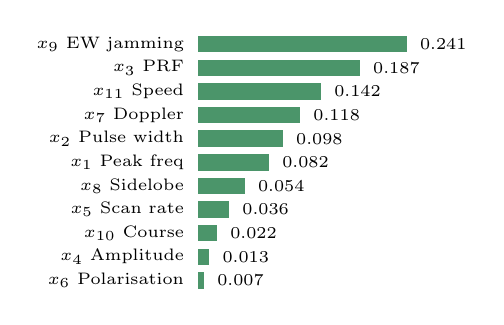
\begin{tikzpicture}[x=11cm,y=0.3cm]
\foreach \i/\lbl/\v in {0/$x_9$ EW jamming/0.241,1/$x_3$ PRF/0.187,2/$x_{11}$ Speed/0.142,3/$x_7$ Doppler/0.118,4/$x_2$ Pulse width/0.098,5/$x_1$ Peak freq/0.082,6/$x_8$ Sidelobe/0.054,7/$x_5$ Scan rate/0.036,8/$x_{10}$ Course/0.022,9/$x_4$ Amplitude/0.013,10/$x_6$ Polarisation/0.007}{\fill[AccentCol!80](0,-\i-0.35)rectangle(\v,-\i+0.35);\node[font=\fontsize{5.8}{6}\selectfont,anchor=east]at(-0.005,-\i){\lbl};\node[font=\fontsize{5.8}{6}\selectfont,anchor=west]at(\v+0.004,-\i){\v};}
\end{tikzpicture}}
\begin{rbox}\scriptsize\textbf{Defence advantage --- fully auditable AI:} a commander can ask ``WHY did the system classify this as an Adversary Bomber?'' and receive a sequence of IF--THEN conditions: essential for Rules-of-Engagement compliance. EW jamming is again the single most discriminative feature, consistent with the expert-system finding.\end{rbox}
\end{columns}
\end{frame}

\sect{7. Random Forest}
\begin{frame}{Random Forest --- Strength in Diversity: Many Weak Learners $\to$ One Strong Classifier}
\begin{columns}[T]
\column{0.55\textwidth}
\figc{3.3cm}{\begin{tikzpicture}
\node[ndN,minimum width=1.5cm](d)at(0,0){$D_\text{train}$\\$N=5{,}780$};
\foreach \i/\y in {1/1.5,2/0.5,3/-0.5,4/-1.5}{\node[nds,minimum width=1.5cm](b\i)at(2.4,\y){bootstrap $D_\i$};\node[ndG,minimum width=1.3cm](t\i)at(4.6,\y){Tree $T_\i$\\\sm{$m=3$ feat./split}};\draw[arr](d)--(b\i);\draw[arr](b\i)--(t\i);}
\node[ndA,minimum width=1.4cm,minimum height=1.6cm](v)at(6.9,0){majority\\vote\\$\hat y$};\foreach \i in {1,2,3,4}{\draw[arr](t\i)--(v);}
\end{tikzpicture}}
\begin{cbox}{Bagging algorithm}\scriptsize \textbf{1.} Draw $B$ bootstrap samples (with replacement; $\approx$63.2\% unique per sample; the rest are out-of-bag, OOB). \textbf{2.} Train $B$ deep trees; at each node consider ONLY $m=\sqrt d=\sqrt{11}\approx3$ random features --- this \emph{decorrelates} the trees. \textbf{3.} Predict by majority vote.\end{cbox}
\column{0.43\textwidth}
\begin{fbx}{Vote and variance reduction}\[\hat y=\arg\max_c\sum_{b=1}^{B}\mathbb{1}[\hat y_b(x)=c]\]\[\text{Var}_{\text{ens}}=\rho\sigma^{2}+\frac{(1-\rho)\sigma^{2}}{B}\]\end{fbx}
\begin{tl}\item Bias stays the same; variance falls toward $\rho\sigma^2$ --- so keep tree correlation $\rho$ low\item \textbf{OOB error} $\approx$ validation error (free!)\item Hyper-parameters: $B$ (100--2000), $m$ ($\sqrt d$ or $d/3$), max depth (usually unlimited), min leaf (1--10)\end{tl}
\end{columns}
\end{frame}

\begin{frame}{Random Forest --- Results on the IADS Data}
\begin{columns}[T]
\column{0.50\textwidth}
\subhead{Tuned: $B=500$, $m=3$, depth $\infty$, min leaf 2}
\figc{3.1cm}{\scriptsize\renewcommand{\arraystretch}{1.15}\begin{tabular}{lccc}\toprule\textbf{Class}&Precision&Recall&F1\\\midrule FF&0.968&0.981&0.974\\AB&0.974&0.961&0.967\\CM&0.978&0.972&0.975\\UV&0.969&0.975&0.972\\CI&0.985&0.989&0.987\\\midrule\textbf{Macro F1}&&&\textbf{0.975}\\\bottomrule\end{tabular}}
\begin{tl}\item Overall \textbf{97.5\%}; OOB error 2.7\% (matches test error!)\item Training 12.4 s (500 trees in parallel); inference 2.8 ms\end{tl}
\column{0.48\textwidth}
\figc{2.6cm}{\begin{tikzpicture}\begin{axis}[ybar,width=7.0cm,height=3.3cm,symbolic x coords={FF,AB,CM,UV,CI},xtick=data,ymin=0.85,ymax=1.0,bar width=7pt,enlarge x limits=0.15,legend style={at={(0.5,1.02)},anchor=south,legend columns=3},ymajorgrids]
\addplot[fill=ISSAblue!60]coordinates{(FF,0.968)(AB,0.974)(CM,0.978)(UV,0.969)(CI,0.985)};\addlegendentry{Precision}
\addplot[fill=AccentCol!80]coordinates{(FF,0.981)(AB,0.961)(CM,0.972)(UV,0.975)(CI,0.989)};\addlegendentry{Recall}
\addplot[fill=ISSAamb!80]coordinates{(FF,0.974)(AB,0.967)(CM,0.975)(UV,0.972)(CI,0.987)};\addlegendentry{F1}
\end{axis}\end{tikzpicture}}
\begin{cbox}[ISSAnavy]{Permutation importance (consistent with a single tree)}\scriptsize EW jamming \textbf{0.228}, PRF \textbf{0.194}, speed \textbf{0.147}.\end{cbox}
\begin{rbox}\scriptsize RF is the accuracy winner for tabular defence classification: robust, low overfit, importances for free.\end{rbox}
\end{columns}
\end{frame}

\sect{8. Gradient Boosting}
\begin{frame}{Gradient Boosting \& XGBoost --- Learning from Residuals}
\begin{columns}[T]
\column{0.55\textwidth}
\figc{1.8cm}{\begin{tikzpicture}\node[nd](f0)at(0,0){$F_0$\\\sm{initial}};\foreach \i/\x in {1/2.0,2/3.9,3/5.8}{\node[ndG](t\i)at(\x,0){tree $T_\i$\\\sm{fit residuals}};}\node[ndA](f)at(8.0,0){$F=F_0+\eta\sum T_m$};
\draw[arr](f0)--(t1);\draw[arr](t1)--(t2);\draw[arr](t2)--(t3);\draw[arr](t3)--(f);\node[lab]at(3.9,-0.8){each tree corrects the errors of the ensemble so far};\end{tikzpicture}}
\begin{cbox}[ISSAnavy]{Boosting vs bagging}\scriptsize \textbf{Bagging (RF):} trees in PARALLEL, independent; reduces VARIANCE; each tree sees $\sim$63\% of data. \textbf{Boosting:} trees SEQUENTIAL; each corrects errors of the previous ensemble; reduces BIAS (also variance).\end{cbox}
\begin{fbx}{Gradient boosting (Friedman 2001)}\[r_{im}=y_i-F_{m-1}(x_i),\qquad F_m(x)=F_{m-1}(x)+\eta\,T_m(x)\]\[F(x)=F_0+\eta\sum_{m=1}^{M}T_m(x)\]\end{fbx}
\column{0.43\textwidth}
\begin{cbox}[ISSAgrn]{XGBoost improvements}\scriptsize $+$ second-order Taylor expansion of the loss; $+$ L1/L2 regularisation on tree structure; $+$ column subsampling per split; $+$ parallel (histogram) split finding.\end{cbox}
\begin{cbox}{Tuned XGBoost and test results}\scriptsize $M=400$, $\eta=0.05$, depth 5, subsample 0.8, colsample 0.8, $\alpha=0.1$, $\lambda=1.0$. \textbf{Accuracy 96.4\%}, macro-F1 0.963, \textbf{AB recall 96.8\%} (vs LR's 87.4\%); training 18.6 s; inference \textbf{0.7 ms}.\end{cbox}
\begin{ibox}\scriptsize \textbf{Vs RF:} RF is slightly more accurate (97.5\% vs 96.4\%); XGBoost has faster inference (0.7 vs 2.8 ms) and a smaller model (better for embedded), but more hyper-parameters. \textbf{Rule of thumb:} tabular $\to$ XGBoost/RF; raw image/signal $\to$ CNN; sequence $\to$ LSTM/Transformer.\end{ibox}
\end{columns}
\end{frame}

\sect{9. Support Vector Machines}
\begin{frame}{SVM --- Maximum-Margin Classifier: Hard-Margin Formulation}
\begin{columns}[T]
\column{0.50\textwidth}
\figc{3.5cm}{\begin{tikzpicture}[x=0.9cm,y=0.9cm]
\draw[ISSAgrey](0,0)rectangle(5,4);
\foreach \x/\y in {0.6/3.4,1.2/2.9,0.7/2.3,1.7/3.5,1.9/2.6}{\node[pt1]at(\x,\y){};}\foreach \x/\y in {3.3/0.5,4.1/1.1,3.8/0.4,4.4/1.7,3.0/1.3}{\node[pt2]at(\x,\y){};}
\draw[AccentCol,line width=1.3pt](0.7,0.2)--(4.4,3.8);\draw[AccentCol,dashed](0.2,0.5)--(3.9,4.1);\draw[AccentCol,dashed](1.2,-0.1)--(4.9,3.5);
\draw[ISSAgrn,thick](2.0,2.65)circle(0.2);\draw[ISSAgrn,thick](3.0,1.3)circle(0.2);\draw[ISSAgrn,thick](1.9,2.6)circle(0.22);
\draw[<->,ISSAnavy](1.55,3.0)--(2.15,2.45)node[midway,right,lab]{margin $2/\|w\|$};
\node[lab,anchor=west]at(0.1,-0.3){\textcolor{ISSAgrn}{circles = support vectors} \quad solid: $w^{\top}x+b=0$};
\end{tikzpicture}}
\begin{fbx}{Hard-margin primal}\[\min_{w,b}\tfrac12\|w\|^{2}\quad\text{s.t.}\quad y_i(w^{\top}x_i+b)\ge1\ \ \forall i\]\end{fbx}
\column{0.48\textwidth}
\begin{fbx}{Dual problem and solution}\[\max_{\alpha}\sum_i\alpha_i-\tfrac12\sum_{i,j}\alpha_i\alpha_jy_iy_jx_i^{\top}x_j\]\[w^{*}=\sum_i\alpha_i^{*}y_ix_i,\qquad\hat y=\text{sign}\Big(\sum_i\alpha_iy_ix_i^{\top}x+b\Big)\]\end{fbx}
\begin{cbox}[ISSAnavy]{Why maximum margin matters in defence}\scriptsize Many hyperplanes separate AB from FF signals; SVM picks the ONE farthest from both clusters --- the most robust to sensor noise, slight adversary variation in signature, and PRF/frequency measurement error.\end{cbox}
\begin{tl}\item $\checkmark$ only support vectors matter (sparse); unique optimum (convex QP)\item $\checkmark$ depends only on dot products $x_i^{\top}x_j\Rightarrow$ \textbf{kernel trick}\item $\times$ fails if not linearly separable $\Rightarrow$ soft margin\end{tl}
\end{columns}
\end{frame}

\begin{frame}{SVM --- Soft Margin \& the $C$ Hyperparameter}
\begin{columns}[T]
\column{0.50\textwidth}
\figc{2.5cm}{\begin{tikzpicture}[x=0.8cm,y=0.8cm]
\draw[ISSAgrey](0,0)rectangle(5,3.4);
\foreach \x/\y in {0.6/2.9,1.2/2.5,0.8/1.8,1.6/3.0}{\node[pt1]at(\x,\y){};}\foreach \x/\y in {3.5/0.6,4.1/1.3,3.8/0.3,4.4/0.9}{\node[pt2]at(\x,\y){};}
\node[pt2]at(1.8,2.0){};\node[pt1]at(3.0,1.0){};\node[pt2]at(2.3,2.3){};
\draw[AccentCol,line width=1.3pt](0.9,0.1)--(4.2,3.3);\draw[AccentCol,dashed](0.5,0.4)--(3.8,3.5);\draw[AccentCol,dashed](1.4,-0.2)--(4.7,3.0);
\node[lab,ISSAred,anchor=west]at(1.9,1.6){$\xi>1$: misclassified};\node[lab,ISSAamb,anchor=west]at(3.1,0.65){$0<\xi<1$: inside margin};
\end{tikzpicture}}
\begin{fbx}{Soft-margin primal (slack $\xi_i\ge0$)}\[\min\ \tfrac12\|w\|^{2}+C\sum_i\xi_i\quad\text{s.t.}\ y_i(w^{\top}x_i+b)\ge1-\xi_i\]\end{fbx}
\begin{tl}\item $\xi_i=0$: correct, outside margin; $0<\xi_i<1$: inside margin, correct side; $\xi_i>1$: misclassified\item Small $C$: more violations, wide margin, may underfit; large $C$: narrow margin, may overfit; $C=\infty$: hard margin\end{tl}
\column{0.48\textwidth}
\subhead{Tuning $C$ (IADS, RBF kernel)}
\figc{2.5cm}{\begin{tikzpicture}\begin{axis}[width=6.6cm,height=3.2cm,xmode=log,xlabel={$C$},ylabel={val. accuracy (\%)},xmin=0.005,xmax=20000,ymin=70,ymax=100,ymajorgrids]
\addplot[AccentCol,thick,mark=*,mark size=1.2pt]coordinates{(0.01,74.2)(0.1,84.6)(1,91.3)(10,94.8)(100,95.4)(1000,95.1)(10000,93.8)};
\node[font=\tiny,ISSAgrn,anchor=south]at(axis cs:100,95.6){optimal $C{=}100$};
\end{axis}\end{tikzpicture}}
\figc{2.2cm}{\scriptsize\renewcommand{\arraystretch}{1.1}\begin{tabular}{lccc}\toprule Class&Prec&Rec&F1\\\midrule FF&0.961&0.973&0.967\\AB&0.967&0.952&0.959\\CM&0.971&0.965&0.968\\UV&0.958&0.961&0.960\\CI&0.978&0.984&0.981\\\bottomrule\end{tabular}}
\sm{Macro F1 0.967; overall 96.7\%; 1,247 SVs (21.6\% of training data); training 38.4 s; inference 4.1 ms}
\end{columns}
\begin{wbox}\scriptsize\textbf{Defence implication:} with asymmetric costs (missing an AB is worse than a false alarm) use class-weighted $C$: $C_{AB}=5\times C_{\text{others}}$. Penalty is not equal across all violations.\end{wbox}
\end{frame}

\begin{frame}{SVM --- The Kernel Trick: Non-linear Classification via Implicit Feature Maps}
\begin{columns}[T]
\column{0.50\textwidth}
\figc{2.4cm}{\begin{tikzpicture}[x=0.55cm,y=0.55cm]
\draw[->](0,0)--(6,0)node[right,font=\tiny]{$x$};\foreach \x in {2.3,2.7,3.0,3.3,3.7}{\node[pt1]at(\x,0){};}\foreach \x in {0.6,1.0,5.0,5.4}{\node[pt2]at(\x,0){};}\node[lab]at(3,-0.7){1-D: not linearly separable};
\draw[bigarr](6.7,1.0)--(8.0,1.0)node[midway,above,font=\tiny]{$\phi$};
\begin{scope}[xshift=8.6cm]\draw[->](0,0)--(6,0)node[right,font=\tiny]{$x$};\draw[->](0,0)--(0,4.2)node[above,font=\tiny]{$x^{2}$};\foreach \x in {2.3,2.7,3.0,3.3,3.7}{\pgfmathsetmacro{\yy}{(\x-3)^2*0.5+0.2}\node[pt1]at(\x,\yy){};}\foreach \x in {0.6,1.0,5.0,5.4}{\pgfmathsetmacro{\yy}{(\x-3)^2*0.5+0.2}\node[pt2]at(\x,\yy){};}\draw[AccentCol,thick](0,1.6)--(6,1.6);\node[lab]at(3,-0.7){2-D: separable by a line};\end{scope}
\end{tikzpicture}}
\begin{fbx}{Kernel function}\[K(x_i,x_j)=\phi(x_i)^{\top}\phi(x_j)\]\end{fbx}
\begin{tl}\item Dot product in a higher-dimensional space \textbf{without} ever computing $\phi(x)$\item \textbf{Linear:} $x^{\top}x'$\quad \textbf{Polynomial:} $(x^{\top}x'+c)^{d}$; $d=2$ maps $\mathbb{R}^{11}\to\mathbb{R}^{78}$\item \textbf{RBF:} $\exp(-\gamma\|x-x'\|^{2})$; $\gamma$ small = smooth, large = sharp\end{tl}
\column{0.48\textwidth}
\subhead{RBF grid search: validation accuracy (\%)}
\figc{2.8cm}{\begin{tikzpicture}[x=1.15cm,y=0.5cm]
\foreach \gi/\g/\a/\b/\cc/\d in {0/0.001/81.2/83.7/85.2/85.3,1/0.01/88.4/91.2/93.8/93.9,2/0.08/91.3/94.8/95.4/95.1,3/0.5/88.7/90.1/92.3/91.8,4/2.0/74.2/75.8/76.4/76.1}{\node[font=\scriptsize\bfseries,anchor=east]at(-0.45,-\gi){$\gamma{=}\g$};\foreach \ci/\v in {0/\a,1/\b,2/\cc,3/\d}{\pgfmathsetmacro{\pp}{(\v-70)*3.4}\node[fill=ISSAgrn!\pp!white,minimum width=1.1cm,minimum height=0.45cm,font=\scriptsize,inner sep=1pt]at(\ci,-\gi){\v};}}
\foreach \ci/\cl in {0/1,1/10,2/100,3/1000}{\node[font=\scriptsize\bfseries]at(\ci,0.6){$C{=}\cl$};}
\draw[ISSAred,line width=1.2pt](1.55,-1.5)rectangle(2.45,-2.5);
\end{tikzpicture}}
\begin{rbox}\scriptsize Optimum $\gamma=0.08$, $C=100$: \textbf{95.4\%}. Large $\gamma=1.0$: 74.1\% (too local, overfit); small $\gamma=0.01$: 89.2\% (too smooth).\end{rbox}
\begin{cbox}[ISSAnavy]{Mercer \& defence-specific kernels}\scriptsize Valid iff $K$ symmetric PSD. \textbf{Spectral:} $\exp(-\|\text{FFT}(x)-\text{FFT}(y)\|^2/2\sigma^2)$. \textbf{DTW:} $\exp(-\text{DTW}(x,y)/\sigma)$ --- speed-invariant tracks. \textbf{String:} shared $k$-grams for SIGINT intercepts.\end{cbox}
\end{columns}
\end{frame}

\sect{10. Naive Bayes}
\begin{frame}{Na\"ive Bayes --- Prior $\times$ Likelihood = Posterior}
\begin{columns}[T]
\column{0.50\textwidth}
\begin{fbx}{Bayes' theorem + independence assumption}\[P(y{=}c|x)\ \propto\ P(y{=}c)\prod_{j=1}^{d}P(x_j|y{=}c)\]\[P(x_j|y{=}c)=\mathcal{N}(x_j;\mu_{cj},\sigma_{cj}^{2})\]\[\hat y=\arg\max_c\Big[\log P(y{=}c)+\sum_j\log P(x_j|y{=}c)\Big]\]\end{fbx}
\begin{tl}\item ``Each feature is conditionally independent given the class'' --- almost never true, yet often works\item Training = class means \& variances: $O(Nd)$; $\approx$0.03 s for IADS\end{tl}
\begin{cbox}[ISSAred]{Test results (Gaussian NB)}\scriptsize Overall accuracy \textbf{83.1\%}, macro-F1 0.826, AB recall \textbf{79.3\%} --- the lowest of all classifiers.\end{cbox}
\column{0.48\textwidth}
\subhead{Worked example: PRF = 1,950 Hz (AB vs FF)}
\figc{2.6cm}{\begin{tikzpicture}\begin{axis}[width=6.6cm,height=3.2cm,xlabel={PRF (Hz)},ylabel={density},xmin=300,xmax=3300,domain=300:3300,samples=80,ticks=none,legend pos=north east]
\addplot[ISSAblue,thick,fill=ISSAblue!15]{exp(-((x-1040)/185)^2/2)/185/2.5066};\addlegendentry{FF: $\mu{=}1040,\sigma{=}185$}
\addplot[ISSAred,thick,fill=ISSAred!12]{exp(-((x-2280)/310)^2/2)/310/2.5066};\addlegendentry{AB: $\mu{=}2280,\sigma{=}310$}
\draw[AccentCol,thick,dashed](axis cs:1950,0)--(axis cs:1950,0.0016);\node[font=\tiny,AccentCol,anchor=south]at(axis cs:1950,0.0016){new signal 1,950};
\end{axis}\end{tikzpicture}}
\begin{tl}\item FF: $z=(1950-1040)/185=4.92\Rightarrow P\approx4.7\times10^{-7}$ --- very unlikely\item AB: $z=(1950-2280)/310=-1.065\Rightarrow P\approx0.0023$ --- far more plausible\item $\Rightarrow$ classifier strongly favours \textbf{AB}: correct!\end{tl}
\begin{wbox}\scriptsize \textbf{Fails when:} strong feature correlations (PRF and speed correlate for AB), non-Gaussian class-conditionals, important interactions. \textbf{Works for:} text, fast baselines, small data, streaming.\end{wbox}
\end{columns}
\end{frame}

\sect{11. Multi-class \& Imbalance}
\begin{frame}{Multi-class Classification Strategies --- Extending Binary Classifiers to 5 Classes}
\figc{2.7cm}{\begin{tikzpicture}
\begin{scope}\node[font=\scriptsize\bfseries,AccentCol]at(1.6,2.2){ONE vs REST (OvR)};\foreach \i/\n in {0/FF,1/AB,2/CM,3/UV,4/CI}{\node[nds,minimum width=2.2cm]at(1.6,1.55-\i*0.42){$f_{\n}$ vs ALL};}\node[lab]at(1.6,-0.7){5 classifiers; predict $\arg\max_c f_c(x)$};\end{scope}
\begin{scope}[xshift=5.2cm]\node[font=\scriptsize\bfseries,AccentCol]at(1.2,2.2){ONE vs ONE (OvO)};\foreach \i in {0,...,4}{\pgfmathsetmacro{\an}{90+72*\i}\node[circle,draw=ISSAnavy,fill=ISSAlblue!50,inner sep=1.5pt,font=\tiny](p\i)at({1.2+0.9*cos(\an)},{0.8+0.9*sin(\an)}){\i};}\foreach \i in {0,...,3}{\foreach \jj in {\i,...,4}{\ifnum\i<\jj\draw[ISSAgrey](p\i)--(p\jj);\fi}}\node[lab]at(1.2,-0.7){$C(C{-}1)/2=10$ classifiers; most wins};\end{scope}
\begin{scope}[xshift=9.6cm]\node[font=\scriptsize\bfseries,AccentCol]at(1.6,2.2){DIRECT MULTI-CLASS};\node[ndN,minimum width=2.2cm,minimum height=1.2cm]at(1.6,0.9){Softmax / tree / RF / NB:\\native $C$-way output};\node[lab]at(1.6,-0.7){best practice: use native when available};\end{scope}
\end{tikzpicture}}
\begin{columns}[T]
\column{0.38\textwidth}
\begin{cbox}[ISSAnavy]{Trade-offs and IADS results}\scriptsize OvR: simple, parallel; but each sub-problem is imbalanced (1 vs 4). OvO: balanced sub-problems; but 10 classifiers for 5 classes (45 for 10). LR: OvR \textbf{89.7\%}, OvO 90.1\%, softmax 89.9\%. SVM with OvO: \textbf{96.7\%}. RF/tree: native.\end{cbox}
\column{0.30\textwidth}
\begin{cbox}[ISSAgrn]{Calibrated probabilities}\scriptsize Raw scores $\neq$ probabilities. \textbf{Platt scaling} (SVM): sigmoid on scores; \textbf{isotonic regression}: monotone fit. A commander needs ``80\% confident this is AB'', not just a label.\end{cbox}
\column{0.30\textwidth}
\begin{cbox}[ISSAred]{Reject option ($\theta=0.6$)}\scriptsize If $\max P(y{=}c|x)<\theta$ $\to$ refer to a human analyst. \textbf{4.2\%} of signals sent to humans (98.7\% human accuracy there); system + human combined: \textbf{99.1\%}.\end{cbox}
\end{columns}
\end{frame}

\begin{frame}{Class Imbalance --- When Your Dataset Lies to You}
\begin{columns}[T]
\column{0.46\textwidth}
\subhead{REAL IADS signal distribution vs our balanced set}
\figc{2.3cm}{\bars{100}{1.6}{1.5}{CI Civilian/78.4/ISSAamb,FF Friendly/14.2/ISSAgrn,UV UAV/4.8/violet,CM Missile/1.8/ISSAblue,AB Bomber/0.8/ISSAred}}
\begin{wbox}\scriptsize Training on the real distribution: the model predicts ``Civilian'' for 92\% of signals $\to$ 78.4\%+14.2\% = \textbf{92.6\% accuracy}, yet \textbf{AB recall = 12.3\%} (87.7\% of bombers missed): clinically useless. Loss minimisation simply learns the imbalance.\end{wbox}
\begin{ibox}\scriptsize \textbf{Data pitfall:} accuracy on imbalanced data is MEANINGLESS. Report precision, recall, F1 per class --- a ``98\% accurate'' model may have 0\% recall on the most important class.\end{ibox}
\column{0.52\textwidth}
\subhead{Four fixes}
\figc{1.9cm}{\begin{tikzpicture}[x=0.55cm,y=0.55cm]\draw[ISSAgrey](0,0)rectangle(4,3);\foreach \x/\y in {0.5/0.6,3.2/2.4}{\node[pt2,inner sep=1.4pt]at(\x,\y){};}\foreach \x/\y in {0.4/2.5,1.0/2.0,1.5/2.8,2.2/2.2,2.6/1.0,1.2/1.0,3.1/0.6,3.6/1.6}{\node[pt1]at(\x,\y){};}
\node[pt2,inner sep=1.4pt,draw=black]at(0.5,0.6){};\node[pt2,inner sep=1.4pt,draw=black]at(3.2,2.4){};\foreach \t in {0.25,0.5,0.75}{\node[circle,draw=ISSAred,fill=white,inner sep=1pt]at({0.5+\t*2.7},{0.6+\t*1.8}){};}\node[lab]at(2,-0.35){SMOTE: $x_\text{new}=x_i+\lambda(x_j-x_i)$};\end{tikzpicture}}
\begin{tl}\item \textbf{Oversample (SMOTE):} interpolate between real AB samples; AB 43 $\to$ 1,700 synthetic added; AB recall $12\%\to89\%$\item \textbf{Undersample:} drop CI samples until balanced --- fast but loses majority-class boundary information\item \textbf{Class-weighted loss:} $w_\text{AB}=N/(C\cdot N_\text{AB})=5780/(5\cdot43)=\mathbf{26.9\times}$ (vs 1.0) --- most natural for RF/LR\item \textbf{Threshold shift:} classify AB if $P(\text{AB}|x)>0.15$ instead of 0.5: more false alarms, higher recall --- when FN cost $\gg$ FP cost\end{tl}
\end{columns}
\end{frame}

\sect{12. Algorithm Comparison}
\begin{frame}{Algorithm Comparison --- All Classifiers on the IADS Dataset}
\begin{columns}[T]
\column{0.58\textwidth}
\figc{4.2cm}{\scriptsize\renewcommand{\arraystretch}{1.17}\begin{tabular}{lcccccc}\toprule\textbf{Algorithm}&Train&Test&F1&AB rec.&Train (s)&Infer (ms)\\\midrule Logistic Reg.&95.4\%&89.7\%&0.897&87.4\%&0.8&0.09\\k-NN ($k$=21)&91.8\%&89.8\%&0.894&88.2\%&---&12.2\\Decision Tree ($d$=10)&95.7\%&91.8\%&0.915&90.4\%&0.5&0.15\\\rowcolor{ISSAgrn!22}\textbf{Random Forest} ($B$=500)&99.2\%&\textbf{97.5\%}&\textbf{0.975}&96.1\%&12.4&2.8\\XGBoost ($M$=400)&98.7\%&96.4\%&0.963&\textbf{96.8\%}&18.6&\textbf{0.7}\\SVM (RBF, $C$=100)&97.8\%&96.7\%&0.967&95.2\%&38.4&4.1\\\rowcolor{ISSAred!18}Naive Bayes&89.1\%&83.1\%&0.826&79.3\%&0.03&0.02\\\bottomrule\end{tabular}}
\sm{Balanced test set, $N=1{,}275$ (15\% of 8,500). SVM: 1,247 support vectors.}
\column{0.40\textwidth}
\figc{2.9cm}{\begin{tikzpicture}\begin{axis}[xbar,width=6.0cm,height=4.0cm,symbolic y coords={NB,LR,kNN,DT,SVM,XGB,RF},ytick=data,xmin=70,xmax=100,bar width=5pt,legend style={at={(0.5,1.03)},anchor=south,legend columns=2},xmajorgrids]
\addplot[fill=ISSAblue!65]coordinates{(83.1,NB)(89.7,LR)(89.8,kNN)(91.8,DT)(96.7,SVM)(96.4,XGB)(97.5,RF)};\addlegendentry{Test acc.}
\addplot[fill=ISSAred!65]coordinates{(79.3,NB)(87.4,LR)(88.2,kNN)(90.4,DT)(95.2,SVM)(96.8,XGB)(96.1,RF)};\addlegendentry{AB recall}
\end{axis}\end{tikzpicture}}
\begin{rbox}\scriptsize\textbf{Winner:} Random Forest (97.5\%, AB recall 96.1\%) for accuracy; XGBoost for fastest inference (0.7 ms); decision tree for interpretability.\end{rbox}
\begin{wbox}\scriptsize\textbf{NEVER use Naive Bayes for this task:} AB recall 79.3\% means 20.7\% of adversary bombers are missed!\end{wbox}
\end{columns}
\end{frame}

\sect{13. Evaluation Metrics}
\begin{frame}{Beyond Accuracy --- ROC \& AUC for Defence AI}
\begin{columns}[T]
\column{0.50\textwidth}
\figc{3.9cm}{\begin{tikzpicture}\begin{axis}[width=6.8cm,height=4.4cm,xlabel={FPR (false-alarm rate)},ylabel={TPR (recall)},xmin=0,xmax=1,ymin=0,ymax=1,domain=0:1,samples=80,legend pos=south east,ymajorgrids,xmajorgrids]
\addplot[ISSAgrn,thick]{1-(1-x)^499};\addlegendentry{RF (0.998)}
\addplot[ISSAblue,thick]{1-(1-x)^249};\addlegendentry{SVM (0.996)}
\addplot[ISSAamb,thick]{1-(1-x)^26};\addlegendentry{LR (0.963)}
\addplot[ISSAred,thick]{1-(1-x)^10.4};\addlegendentry{NB (0.912)}
\addplot[ISSAgrey,dashed]{x};\addlegendentry{random (0.5)}
\end{axis}\end{tikzpicture}}
\sm{Schematic curves drawn to reproduce the reported AUCs (AB class, one-vs-rest); exact shapes are illustrative.}
\column{0.48\textwidth}
\begin{cbox}[ISSAnavy]{ROC curve \& AUC}\scriptsize At each threshold $\theta$: TPR $=TP/(TP+FN)$ (y), FPR $=FP/(FP+TN)$ (x). Ideal: top-left corner $(0,1)$; random: the diagonal, AUC $=0.5$; AUC below the diagonal means an inverted classifier.\end{cbox}
\figc{2.0cm}{\scriptsize\begin{tabular}{lccccc}\toprule&RF&SVM&LR&DT&NB\\\midrule AUC (AB, OvR)&\textbf{0.998}&0.996&0.963&0.940&0.912\\TPR @ FPR 5\%&\textbf{97.8\%}&96.4\%&88.3\%&---&---\\\bottomrule\end{tabular}}
\begin{ibox}\scriptsize ROC-AUC is best when classes are balanced (lab conditions). On the real imbalanced stream, FPR hides how many alarms are false relative to true threats --- precision--recall is more informative (next slide).\end{ibox}
\end{columns}
\end{frame}

\begin{frame}{Precision--Recall, Average Precision and the $F_\beta$ Score}
\begin{columns}[T]
\column{0.52\textwidth}
\subhead{AB class on real imbalanced data (0.8\% AB)}
\figc{2.4cm}{\begin{tikzpicture}[x=1]\node[font=\scriptsize\bfseries]at(0,0.9){};\end{tikzpicture}\bars{1}{1.6}{1.7}{RF average precision/0.887/ISSAgrn,LR average precision/0.642/ISSAamb,NB average precision/0.441/ISSAred}}
\begin{fbx}{Average precision and $F_\beta$}\[AP=\sum_k(R_k-R_{k-1})P_k,\qquad F_\beta=(1+\beta^2)\frac{PR}{\beta^2P+R}\]\end{fbx}
\begin{tl}\item $\beta>1$ weights recall more (miss cost $>$ false-positive cost); \textbf{$\beta=2$} recommended for the IADS AB class\end{tl}
\column{0.46\textwidth}
\subhead{Operational metrics}
\figc{2.2cm}{\bars{100}{1.5}{2.4}{RF: recall while precision $>$95\%/91.4/ISSAgrn,LR: recall while precision $>$95\%/72.3/ISSAamb}}
\figc{2.1cm}{\bars{1}{1.4}{2.4}{RF $F_2$ (AB)/0.974/ISSAgrn,LR $F_2$ (AB)/0.894/ISSAamb}}
\begin{rbox}\scriptsize\textbf{Operational choice:} use ROC-AUC for balanced (lab) classes; use the P--R curve / AP on real imbalanced data. For the IADS, \textbf{$F_2$ on the AB class} is the primary metric: recall matters twice as much as precision.\end{rbox}
\end{columns}
\end{frame}


\sect{13a. Satellite \& SAR Imagery}
\begin{frame}{Satellite \& SAR Image Interpretation --- Four Tasks, One CNN Backbone}
\begin{columns}[T]
\column{0.47\textwidth}
\subhead{What the analyst needs}
\figc{3.0cm}{\scriptsize\renewcommand{\arraystretch}{1.25}\begin{tabular}{>{\bfseries}l p{2.2cm} p{2.5cm}}\toprule Task & Output & Example\\\midrule
Classification & one label per chip & ``T-72-class tank''\\
Detection & box + label per object & all vehicles in 10 km$^2$\\
Segmentation & label per pixel & roads, buildings, water\\
Change detection & what differs between dates & new revetments since last week\\\bottomrule\end{tabular}}
\begin{ibox}\scriptsize\textbf{Scale problem:} a vehicle may be 10$\times$20 pixels in a 30,000$\times$30,000 scene. Scenes are cut into overlapping tiles; detections are merged across tile edges.\end{ibox}
\begin{tl}\scriptsize\item \textbf{Two-stage} detectors (R-CNN family): propose regions, then classify --- accurate, slower
\item \textbf{One-stage} (YOLO, SSD, RetinaNet): boxes from a grid in one pass --- real-time video
\item \textbf{NMS} removes duplicate overlapping boxes\end{tl}
\column{0.51\textwidth}
\subhead{Detection pipeline}
\figc{4.6cm}{\begin{tikzpicture}[font=\scriptsize,node distance=0.32cm]
\node[nd,text width=2.2cm](sc){Scene\\(EO or SAR)};
\node[nd,below=of sc,text width=2.2cm](ti){Tile into chips\\(overlap 10--20\%)};
\node[ndA,below=of ti,text width=2.2cm](bb){CNN backbone\\(pre-trained, fine-tuned)};
\node[nd,below=of bb,text width=2.2cm](hd){Detection head\\boxes + classes + scores};
\node[nd,below=of hd,text width=2.2cm](nm){NMS + merge tiles};
\node[ndG,right=0.7cm of nm,text width=2.0cm](aq){Ranked analyst queue};
\draw[arr](sc)--(ti);\draw[arr](ti)--(bb);\draw[arr](bb)--(hd);\draw[arr](hd)--(nm);\draw[arr](nm)--(aq);
\node[nd,right=0.7cm of bb,text width=2.0cm](tr){Transfer learning: few thousand labelled chips};
\draw[arr,dashed](tr)--(bb);
\end{tikzpicture}}
\end{columns}
\end{frame}

\begin{frame}{Detection Metrics --- Intersection over Union and Average Precision}
\begin{columns}[T]
\column{0.48\textwidth}
\begin{fbx}{Intersection over union}\[\text{IoU}=\frac{\text{area}(B_{\text{pred}}\cap B_{\text{true}})}{\text{area}(B_{\text{pred}}\cup B_{\text{true}})}\]\end{fbx}
\figc{2.1cm}{\begin{tikzpicture}[scale=0.05,font=\scriptsize]
\fill[ISSAgrn!15](10,10)rectangle(50,50);\draw[ISSAgrn,thick](10,10)rectangle(50,50);
\fill[AccentCol!30](15,15)rectangle(50,50);\draw[AccentCol,thick,dashed](15,15)rectangle(55,55);

\fill[ISSAgrn!15](100,10)rectangle(140,50);\draw[ISSAgrn,thick](100,10)rectangle(140,50);
\fill[AccentCol!30](120,30)rectangle(140,50);\draw[AccentCol,thick,dashed](120,30)rectangle(160,70);

\end{tikzpicture}}
{\scriptsize\hspace*{0.6cm}IoU $=0.62$ \grn{hit}\hspace{2.2cm}IoU $=0.14$ \red{miss}}\par\vspace{2pt}
\sm{True box (solid) 40$\times$40 px. Left: overlap $35^2=1{,}225$, union $1{,}975$. Right: overlap $20^2=400$, union $2{,}800$. A hit needs IoU $\ge0.5$.}
\column{0.50\textwidth}
\subhead{Average precision: 5 vehicles, 8 detections}
\figc{1.0cm}{\scriptsize\begin{tabular}{lcccccccc}\toprule rank&1&2&3&4&5&6&7&8\\\midrule hit?&\grn{H}&\grn{H}&\red{F}&\grn{H}&\red{F}&\grn{H}&\red{F}&\red{F}\\precision&1.00&1.00&0.67&0.75&0.60&0.67&0.57&0.50\\recall&0.2&0.4&0.4&0.6&0.6&0.8&0.8&0.8\\\bottomrule\end{tabular}}
\figc{2.6cm}{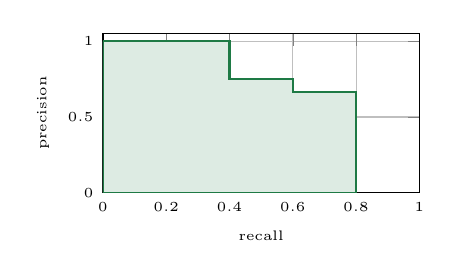
\begin{tikzpicture}\begin{axis}[width=5.6cm,height=3.6cm,xmin=0,xmax=1,ymin=0,ymax=1.05,xlabel={recall},ylabel={precision},grid=major,font=\tiny]
\addplot[fill=AccentCol!15,draw=AccentCol,thick]coordinates{(0,0)(0,1)(0.4,1)(0.4,0.75)(0.6,0.75)(0.6,0.667)(0.8,0.667)(0.8,0)}--cycle;
\end{axis}\end{tikzpicture}}
\begin{rbox}\scriptsize AP $=0.2(1)+0.2(1)+0.2(0.75)+0.2(0.67)=\mathbf{0.68}$. One vehicle never found: recall stops at 0.8. \textbf{mAP} averages AP over classes (and IoU thresholds 0.5--0.95).\end{rbox}
\end{columns}
\end{frame}

\begin{frame}{SAR Is Not a Photograph --- Pitfalls and the Imagery-Triage Concept}
\begin{columns}[T]
\column{0.49\textwidth}
\subhead{Why overhead imagery is hard}
\begin{tl}\scriptsize
\item \textbf{SAR physics:} speckle noise, layover and radar shadow; a vehicle's signature changes with \textbf{look (aspect and depression) angle}
\item \textbf{Distribution shift:} public SAR benchmarks (e.g.\ MSTAR, 10 vehicle classes) give near-perfect accuracy under matched conditions --- and sharp drops when depression angle or vehicle configuration changes
\item \textbf{Arbitrary orientation:} rotated boxes + rotation augmentation
\item \textbf{Change detection:} naive differencing flags shadows, seasons and sensor changes; Siamese CNNs compare deep features of two dates
\item \textbf{Deception:} decoys, camouflage nets, adversarial patterns target exactly these detectors
\end{tl}
\begin{wbox}\scriptsize\textbf{Defence:} multi-sensor confirmation (EO + SAR + SIGINT); test on the deployment sensor and season, never only on the benchmark.\end{wbox}
\column{0.49\textwidth}
\subhead{Operating concept: AI triage, analyst decides}
\figc{3.4cm}{\begin{tikzpicture}[font=\scriptsize]
\node[ndA,text width=2.1cm](d)at(0,0){Detector scores every scene};
\node[nd,text width=2.1cm](r)at(3.3,0){Chips ranked by threat score};
\node[ndG,text width=2.1cm](a)at(3.3,-1.7){Analyst confirms or rejects};
\node[nd,text width=2.1cm](l)at(0,-1.7){New labels; periodic retraining};
\draw[arr](d)--(r);\draw[arr](r)--(a);\draw[arr](a)--(l);\draw[arr](l)--(d);
\end{tikzpicture}}
\begin{rbox}\scriptsize\textbf{Measure success operationally:} analyst hours saved and threats found earlier \emph{at a stated recall} --- not benchmark mAP alone.\end{rbox}
\end{columns}
\end{frame}

\sect{13b. Across Disciplines}
\begin{frame}{Classification Across the Disciplines --- From Radar Scopes to Hospital Wards}
\subhead{The same ideas recur in every science --- and each has a defence application}
\figc{5.0cm}{\begin{tikzpicture}
\tikzset{G/.style={nd,text width=4.75cm,align=left,minimum height=2.3cm,font=\fontsize{6.9}{8.2}\selectfont,inner sep=3pt}}
\node[G,draw=ISSAblue,fill=ISSAblue!7]at(-5,1.25){\textbf{\textcolor{ISSAblue}{AERONAUTICS / RADAR $\to$ PSYCHOLOGY}}\\The ROC curve was born with WWII radar operators deciding ``target or noise''. Signal-detection theory (Peterson, Birdsall \& Fox, 1954) then entered psychophysics (Tanner \& Swets, 1954).\\\textbf{Defence:} every IADS alert threshold is a point on an ROC curve.};
\node[G,draw=ISSAgrn,fill=ISSAgrn!7]at(0,1.25){\textbf{\textcolor{ISSAgrn}{BIOLOGY / MEDICINE}}\\Cancer screening trades sensitivity against false recalls; the operating point is set by the cost of a missed case, not by accuracy.\\\textbf{Defence:} recall-first thresholds for the rare Adversary-Bomber class (Lecture 2 case study).};
\node[G,draw=ISSAred,fill=ISSAred!6]at(5,1.25){\textbf{\textcolor{ISSAred}{ENGINEERING}}\\Vibration signatures classify bearing and gearbox faults before failure --- the basis of helicopter health \& usage monitoring (HUMS).\\\textbf{Defence:} fleet availability; ``healthy vs incipient fault'' with heavy class imbalance.};
\node[G,draw=violet,fill=violet!7]at(-5,-1.25){\textbf{\textcolor{violet}{PSYCHOLOGY}}\\Meehl (1954), \textit{Clinical versus Statistical Prediction}: simple actuarial rules matched or beat expert judgement in most comparisons.\\\textbf{Defence:} structured classifiers can outperform unaided gut calls on track ID --- with a human still accountable.};
\node[G,draw=ISSAamb,fill=ISSAyell!45]at(0,-1.25){\textbf{\textcolor{ISSAamb!80!black}{STATISTICS}}\\Fisher's iris data (1936) introduced linear discriminant analysis --- ancestor of logistic regression and SVM boundaries.\\\textbf{Defence:} separating radar-emitter classes using PRF and pulse width.};
\node[G,draw=AccentCol,fill=AccentCol!8]at(5,-1.25){\textbf{\textcolor{AccentCol}{WARGAMING}}\\Identifying OPFOR unit types from partial, fog-of-war observations; rare but critical classes (HQs, air-defence nodes) need per-class recall and calibrated confidence.\\\textbf{Use:} kNN/RF on observed signatures.};
\end{tikzpicture}}
\begin{ibox}\scriptsize\textbf{Common thread:} a classifier is a decision rule under uncertainty. Choose the threshold from the cost of each error type in \emph{your} mission --- radar operators, physicians and maintenance engineers all learned this the hard way.\end{ibox}
\end{frame}

\sect{14. Summary}
\begin{frame}{Lecture 2 Summary --- Six Classifiers, One Mission}
\figc{4.8cm}{\begin{tikzpicture}
\tikzset{K/.style={nd,text width=3.6cm,align=left,minimum height=2.0cm,font=\fontsize{6.4}{7.6}\selectfont,inner sep=3pt}}
\node[K,draw=ISSAblue,fill=ISSAblue!8]at(-4,1.2){\textbf{LOGISTIC REGRESSION}\\Fast, interpretable (weights); linear boundaries only; baseline for all tasks.\\\textbf{Use:} interpretable baseline or well-separated classes};
\node[K,draw=ISSAgrn,fill=ISSAgrn!8]at(0,1.2){\textbf{kNN ($k=21$)}\\No training; local structure; expensive inference $O(N)$; bias--variance tied to $k$.\\\textbf{Use:} rare events; updatable in real time};
\node[K,draw=ISSAamb,fill=ISSAyell!40]at(4,1.2){\textbf{DECISION TREE ($d=10$)}\\Fully interpretable IF--THEN; axis-aligned boundaries; pruning prevents overfit.\\\textbf{Use:} ROE compliance; commander explainability};
\node[K,draw=AccentCol,fill=AccentCol!12,line width=1.2pt]at(-4,-1.2){\textbf{RANDOM FOREST} \textbf{(winner)}\\97.5\% accuracy, F1 0.975; robust, low overfit; feature importance for free.\\\textbf{Use:} BEST overall for tabular defence classification};
\node[K,draw=violet,fill=violet!8]at(0,-1.2){\textbf{XGBOOST}\\96.4\%; fastest inference 0.7 ms; sequential error correction; many hyper-parameters.\\\textbf{Use:} real-time embedded systems};
\node[K,draw=ISSAred,fill=ISSAred!7]at(4,-1.2){\textbf{SVM (RBF)}\\96.7\%; principled margin; sparse SVs (21.6\%); training $O(N^2$--$N^3)$.\\\textbf{Use:} small--medium datasets needing a margin guarantee};
\end{tikzpicture}}
\end{frame}

\begin{frame}{Looking Ahead --- Lecture 3: Regression \& Multi-Sensor Fusion}
\begin{columns}[T]
\column{0.48\textwidth}
\subhead{Lecture 3 topics}
\begin{tl}\item Linear regression: OLS derivation (closed form)\item Regularised regression: Ridge (L2, shrinks), Lasso (L1, sparsity), Elastic Net\item Support vector regression: $\varepsilon$-insensitive loss; kernel SVR\item Gradient boosting for regression (XGBRegressor on logistics data)\item \textbf{Practical:} casualty estimation; force-effectiveness regression\item \textbf{Sensor fusion:} Kalman filter; ML-enhanced fusion; radar + IR + ELINT (3 sensors, 5 targets); late vs early fusion\item Prediction uncertainty \& Bayesian regression\end{tl}
\begin{ibox}\scriptsize \textbf{Assignment 2} is released with this lecture pack.\end{ibox}
\column{0.50\textwidth}
\subhead{Preview: time-to-mission-completion ($N=6{,}200$, 18 features)}
\figc{2.2cm}{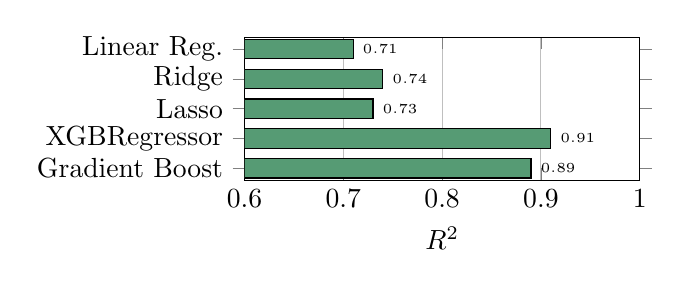
\begin{tikzpicture}\begin{axis}[xbar,width=6.6cm,height=3.4cm,symbolic y coords={Gradient Boost,XGBRegressor,Lasso,Ridge,Linear Reg.},ytick=data,xmin=0.6,xmax=1,bar width=7pt,nodes near coords,nodes near coords style={font=\fontsize{5.5}{6}\selectfont},xlabel={$R^{2}$},xmajorgrids]
\addplot[fill=AccentCol!75]coordinates{(0.89,Gradient Boost)(0.91,XGBRegressor)(0.73,Lasso)(0.74,Ridge)(0.71,Linear Reg.)};
\end{axis}\end{tikzpicture}}
\figc{1.5cm}{\scriptsize\begin{tabular}{lcc}\toprule Model&$R^2$&RMSE (h)\\\midrule Linear&0.71&4.2\\Ridge ($\lambda$=0.8)&0.74&3.9\\Lasso ($\lambda$=0.3)&0.73&4.0\\Gradient boost&0.89&2.3\\\textbf{XGBRegressor}&\textbf{0.91}&\textbf{2.1}\\\bottomrule\end{tabular}}
\begin{cbox}[ISSAnavy]{Fusion preview}\scriptsize 3-sensor (radar + IR + ELINT) track correlation: a single sensor vs a Kalman filter vs ML fusion --- Lecture 3.\end{cbox}
\end{columns}
\end{frame}
\end{document}
